% Project GAIA — System Architecture (TikZ)
% USENIX double-column figure
\begin{figure*}[t]
\centering
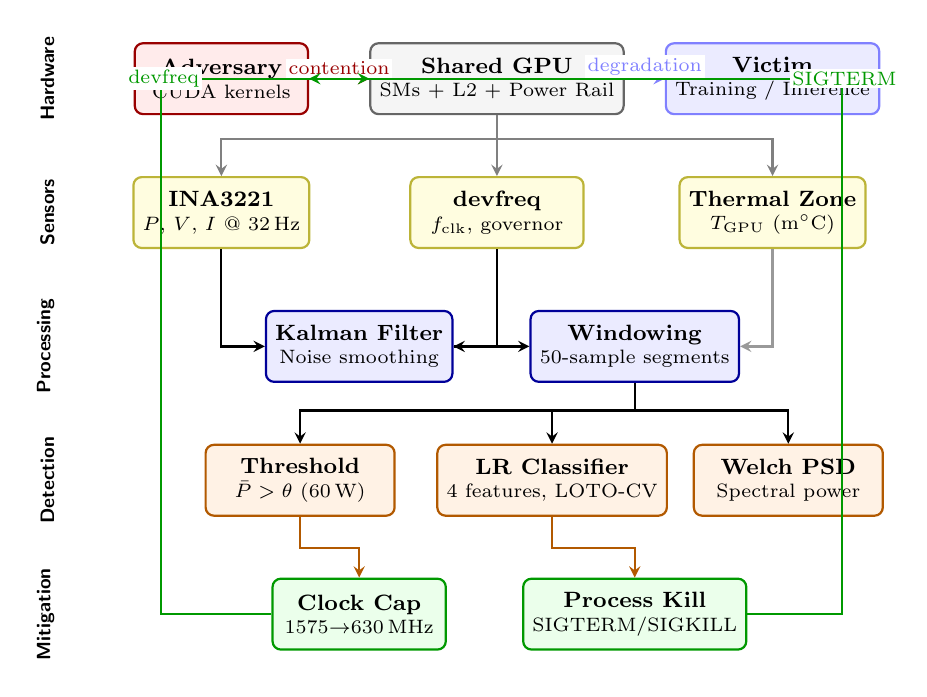
\begin{tikzpicture}[
    >=stealth,
    every node/.style={font=\footnotesize},
    phase/.style={draw, rounded corners=3pt, minimum height=0.9cm,
                  minimum width=2.2cm, align=center, thick, fill=#1},
    phase/.default=white,
    sensor/.style={phase=yellow!12, draw=yellow!70!black},
    proc/.style={phase=blue!8, draw=blue!60!black},
    det/.style={phase=orange!10, draw=orange!70!black},
    mit/.style={phase=green!8, draw=green!60!black},
    attack/.style={phase=red!8, draw=red!60!black},
    arr/.style={->, thick},
    lbl/.style={font=\scriptsize, fill=white, inner sep=1pt},
]

% === Row 1: Hardware Layer ===
\node[attack] at (0,0) (atk) {\textbf{Adversary}\\[-1pt]{\scriptsize CUDA kernels}};
\node[phase=gray!8, draw=black!60, minimum width=3.0cm] at (3.5,0) (gpu)
    {\textbf{Shared GPU}\\[-1pt]{\scriptsize SMs + L2 + Power Rail}};
\node[phase=blue!8, draw=blue!50] at (7.0,0) (vic)
    {\textbf{Victim}\\[-1pt]{\scriptsize Training / Inference}};

\draw[arr, red!60!black] (atk) -- (gpu) node[lbl, midway, above] {contention};
\draw[arr, blue!50] (gpu) -- (vic) node[lbl, midway, above] {degradation};

% === Row 2: Telemetry Layer ===
\node[sensor] at (0,-1.7) (ina) {\textbf{INA3221}\\[-1pt]{\scriptsize $P$, $V$, $I$ @ 32\,Hz}};
\node[sensor] at (3.5,-1.7) (dvfs) {\textbf{devfreq}\\[-1pt]{\scriptsize $f_{\mathrm{clk}}$, governor}};
\node[sensor] at (7.0,-1.7) (therm) {\textbf{Thermal Zone}\\[-1pt]{\scriptsize $T_{\mathrm{GPU}}$ (m$^\circ$C)}};

\draw[arr, black!50] (gpu.south) -- ++(0,-0.3) -| (ina.north);
\draw[arr, black!50] (gpu.south) -- (dvfs.north);
\draw[arr, black!50] (gpu.south) -- ++(0,-0.3) -| (therm.north);

% === Row 3: Processing ===
\node[proc] at (1.75,-3.4) (kalman) {\textbf{Kalman Filter}\\[-1pt]{\scriptsize Noise smoothing}};
\node[proc] at (5.25,-3.4) (window) {\textbf{Windowing}\\[-1pt]{\scriptsize 50-sample segments}};

\draw[arr] (ina.south) |- (kalman.west);
\draw[arr] (dvfs.south) |- (kalman.east);
\draw[arr] (kalman) -- (window);
\draw[arr, black!40] (therm.south) |- (window.east);

% === Row 4: Detection ===
\node[det, minimum width=2.4cm] at (1.0,-5.1) (thresh)
    {\textbf{Threshold}\\[-1pt]{\scriptsize $\bar{P} > \theta$ (60\,W)}};
\node[det, minimum width=2.4cm] at (4.2,-5.1) (lr)
    {\textbf{LR Classifier}\\[-1pt]{\scriptsize 4 features, LOTO-CV}};
\node[det, minimum width=2.4cm] at (7.2,-5.1) (spectral)
    {\textbf{Welch PSD}\\[-1pt]{\scriptsize Spectral power}};

\draw[arr] (window.south) -- ++(0,-0.35) -| (thresh.north);
\draw[arr] (window.south) -- ++(0,-0.35) -| (lr.north);
\draw[arr] (window.south) -- ++(0,-0.35) -| (spectral.north);

% === Row 5: Mitigation ===
\node[mit, minimum width=2.2cm] at (1.75,-6.8) (cap)
    {\textbf{Clock Cap}\\[-1pt]{\scriptsize 1575$\to$630\,MHz}};
\node[mit, minimum width=2.2cm] at (5.25,-6.8) (kill)
    {\textbf{Process Kill}\\[-1pt]{\scriptsize SIGTERM/SIGKILL}};

\draw[arr, orange!70!black] (thresh.south) |- ++(0,-0.4) -| (cap.north);
\draw[arr, orange!70!black] (lr.south) |- ++(0,-0.4) -| (kill.north);

% Feedback to GPU
\draw[arr, green!60!black, thick]
    (cap.west) -- ++(-1.4,0) |- (gpu.west)
    node[lbl, pos=0.6, left] {\scriptsize devfreq};
\draw[arr, green!60!black, thick]
    (kill.east) -- ++(1.2,0) |- (atk.east)
    node[lbl, pos=0.55, right] {\scriptsize SIGTERM};

% === Layer labels ===
\node[font=\scriptsize\sffamily\bfseries, rotate=90, anchor=south]
    at (-2.0,0) {Hardware};
\node[font=\scriptsize\sffamily\bfseries, rotate=90, anchor=south]
    at (-2.0,-1.7) {Sensors};
\node[font=\scriptsize\sffamily\bfseries, rotate=90, anchor=south]
    at (-2.0,-3.4) {Processing};
\node[font=\scriptsize\sffamily\bfseries, rotate=90, anchor=south]
    at (-2.0,-5.1) {Detection};
\node[font=\scriptsize\sffamily\bfseries, rotate=90, anchor=south]
    at (-2.0,-6.8) {Mitigation};

\end{tikzpicture}
\caption{GAIA system architecture.  Hardware telemetry from INA3221
current sensors, devfreq clock state, and GPU thermal zones feeds a
Kalman-filtered processing pipeline.  Non-overlapping 50-sample windows
are classified by a power-level threshold detector and a logistic
regression classifier (4~features, LOTO-CV); Welch PSD provides spectral
characterization.  Anomaly detection triggers either devfreq clock
capping (Strategy~A) or adversarial process termination (Strategy~B).}
\label{fig:sysarch}
\end{figure*}
